\section{General-purpose Counterfactuals}
\label{sec:general_purpose}


%\hao{a road map here would help}
\begin{comment}
* Define the task
- Some math
- Several different application domains
    - augmentation
    - adversarial attack
    - extend data
    - counterfactual explanation
- Importance of where to change and how to change

* How to train
- Compute control tags
- Special tokens

* Use existing datasets
- Why each dataset 
- Data distribution [maybe appendix]

* Training hyperparameters

* Evaluations
- Filtering
- Diversity
\end{comment}

\begin{comment}
% Originally wanted a table to summarize 
\begin{table}
\small
\centering
\begin{tabular}{r c c}
\toprule

Application & \textbf{$y = \yp$} & $f(x)=f(\xp)$ \\ 
\midrule
Adversarial training 		& \cmark & \qmark \\
Data augmentation  			& \qmark & \qmark \\
Perturbation explanation 	& \qmark & \qmark \\
Adversarial training 		& \cmark & \qmark \\
\bottomrule
\end{tabular}

\caption{The datasets used for finetuning the GPT-2 perturbation model, and the \tagstr distributions.}
\label{table:gpt_train_stats}
\end{table}
\end{comment}


\textbf{Definition.}
Given an instance $x \in \xset$, a counterfactual generator $g$ should produce a set of counterfactuals $\hat{\xset} = \{\xp_1, \xp_2, ...\}$ with varying relationships $x \rightarrow \xp$ (referred as $\relation{\xp_i}$ for simplicity).
% Each $\xp_i$ perturbs $x$ with certain strategies like negations, syntactic restructuring, etc., and the edited spans are instantiations of the strategies.
For example, \swap{great}{not great}, \swap{kids}{no one} in Figure~\ref{fig:teaser} are both instances of the \ctrltag{negation} relationship.
Considering the \emph{label} relationship, both instances \emph{flip the groundtruth}, but the \emph{model prediction is intact} on the latter\footnote{All examples shown are actual generations of \sysname.}.
Another example of a lower level relationship would be \emph{the word ``kids'' is replaced}, \eg \swap{kids}{no one} and \swap{kids}{adults}.

As illustrated in \S\ref{sec:desiderata} below, we summarize from social science research that the $\hat{\xset}$ should cover (1) \emph{diverse} $\xp$, and each $\xp$ should be (2) \emph{fluent} and (3) \emph{close} to $x$, regardless of the applications; Whereas the relevant relationship $\relation{\xp}$ would vary with applications.
The three desiderate inspire our modeling in \S\ref{subsec:nlg}, including the training prompt design, datasets, and filtering strategies.


% on a particular instance
% 
\subsection{Desiderata}
\label{sec:desiderata}

% Knowledge of such relationships aid downstream filtering and ranking.
% $\relation{\xp}$ then forms certain relationships that are useful for downstream filtering (\eg perturbation strategy, the added and removed tokens, the impacts on groundtruth label, model prediction, etc.)
%The perturbation follow certain \emph{strategies} $s$ (e.g., negations~\cite{kaushik2019learning}, word substitution~\cite{li-etal-2020-bert-attack}, syntactical restructing~\cite{iyyer2018adversarial}).

%Desired counterfactuals are usually~\cite{morris2020textattack}:
\textbf{Individual counterfactuals.} 
A counterfactual $\xp$ should be \emph{close} to $x$, preferably only involving the minimal changes necessary for establishing a certain effect while leaving the rest of the instance intact~\cite{pearl2018causal}, allowing users to make causality assessments from $\relation{\xp}$. 
If we add negation \emph{and} remove a clause from a particular $x$ simultaneously, it is unclear which change should the resulting behavior be attributed to. 
It has long been observed that humans strongly favor counterfactuals that are closer to the original instance~\cite{kahneman}, even when the same variable is acted upon.
NLP research usually estimate \emph{closeness} using the semantic and syntactic distance between $x$ and $\xp$~\cite{morris2020textattack, madaan2020generate}.

However, $\xp$ also needs to be realistic, \ie the counterfactual scenario should be one that could have easily happened, without rare assumptions or coincidences~\cite{kahneman}. 
In NLP, this translates to \emph{fluent} counterfactuals that are grammatically correct~\cite{morris2020textattack} and semantically meaningful (\eg \exinline{It's scary for water} is grammatically correct but not meaningful.) 

\textbf{Sets of counterfactuals.} There can be infinite numbers of ``what-ifs''~\cite{pearl2018causal, kahneman}, especially as we allow $\xp$ to deviate from $x$. Since our goal is to produce a general-purpose set of counterfactuals, we expect the set to be \emph{diverse} in terms of relationships between $x$ and $\xp$.
However, when the targeted relationship is unclear, an approximation could be the similarity of counterfactuals \emph{to each other} (using \eg self-BLEU~\cite{Hu2017TowardCG}).
%, and also to contain various instantiations of the same relationship.



%Additionally, augmentations usually prioritize (3) \emph{diversity} --- a group of $x$s are preturbed using various strategies, and various initiations under the same strategy, such that they provide different constraints on finetuning decision boundaries.
%On the other hand, evaluations and explanations require more (4) \emph{controlled} perturbations for systematic and targeted inspections.
%The diversity and the controllability are two competing factors, and prior work focusing on certain applications follow one of two extremes.
%Those that thrive in diversity are either too uncontrolled (\eg text generation~\cite{iyyer2018adversarial}) or hard to scale (\eg manual rewrites~\cite{kaushik2019learning, gardner2020contrast}), whereas those that rely on templates or heuristic rules usually only cover limited linguistic patterns~\cite{li2020linguistically}.



\newcommand{\tagdefine}[1]{\emph{{\color{darkgray}#1} }}
%\renewcommand{\arraystretch}{1.1}
\begin{table*}
\small
\centering
\begin{tabular}{@{} p{0.11\linewidth} p{0.61\linewidth}  p{0.22\linewidth} @{}}
\toprule
\textbf{\Tagstr} & \textbf{Definitions and \sysname-generated Examples} & \textbf{Training datasets} \\ 
\midrule
\ctrltag{negation}
    & A dog is \add{not} embraced by the woman.
    & \cite{kaushik2019learning}
\\ \midrule
\ctrltag{quantifier}
    & \swap{A dog is}{Three dogs are} embraced by the woman. 
    & \cite{gardner2020contrast}
\\ \midrule
\ctrltag{shuffle}
    & \tagdefine{To move (or swap) key phrases or entities around the sentence.} \newline
    A \swap{dog}{woman} is embraced by the \swap{woman}{dog}.
    & \cite{zhang2019paws}
\\ \midrule
\ctrltag{lexical}
    & \tagdefine{Changing just one word or noun chunks without breaking the POS tags.} \newline
      A dog is \swap{embraced}{attacked} by the woman.
    & \cite{sakaguchi2019winogrande}
\\ \midrule
\ctrltag{resemantic}
    & \tagdefine{Replacing short phrases or clauses without affecting the parsing tree.}\newline
      A dog is \swap{embraced by the woman}{wrapped in a blanket}.
    & \cite{sakaguchi2019winogrande}
\\ \midrule
\ctrltag{insert}
    & \tagdefine{Adding constraints without affecting the parsing structure of other parts.} \newline
      A dog is embraced by the \add{little} woman.
    & \cite{mccoy2019right}
\\ \midrule
\ctrltag{delete}
    & \tagdefine{Removing constraints without affecting the parsing structure of other parts.} \newline
    A dog is embraced \remove{by the woman}.
    & \cite{mccoy2019right}
\\ \midrule
\ctrltag{restructure}
    & \tagdefine{Altering the dependency tree structure, \eg changing from passive to positive.} \newline
    A dog is \swap{embraced by}{hugging} the woman.
    & \cite{wieting2017paranmt}
\\
\bottomrule
\end{tabular}
\vspace{-5pt}
\caption{A list of \tagstrs used for semantically driving the counterfactual generation, their corresponding examples, and the representative training datasets for the corresponding patterns. More examples are in \S\ref{appendix:example}.}
%\wts{Change all the examples to be on an identical sentence, not all different cases. And consider further annotate the tags based on whether they just do semantic change or also syntactic change.}}
\label{table:ctrltag}
\vspace{-10pt}
\end{table*}


\begin{figure}[t]
\centering
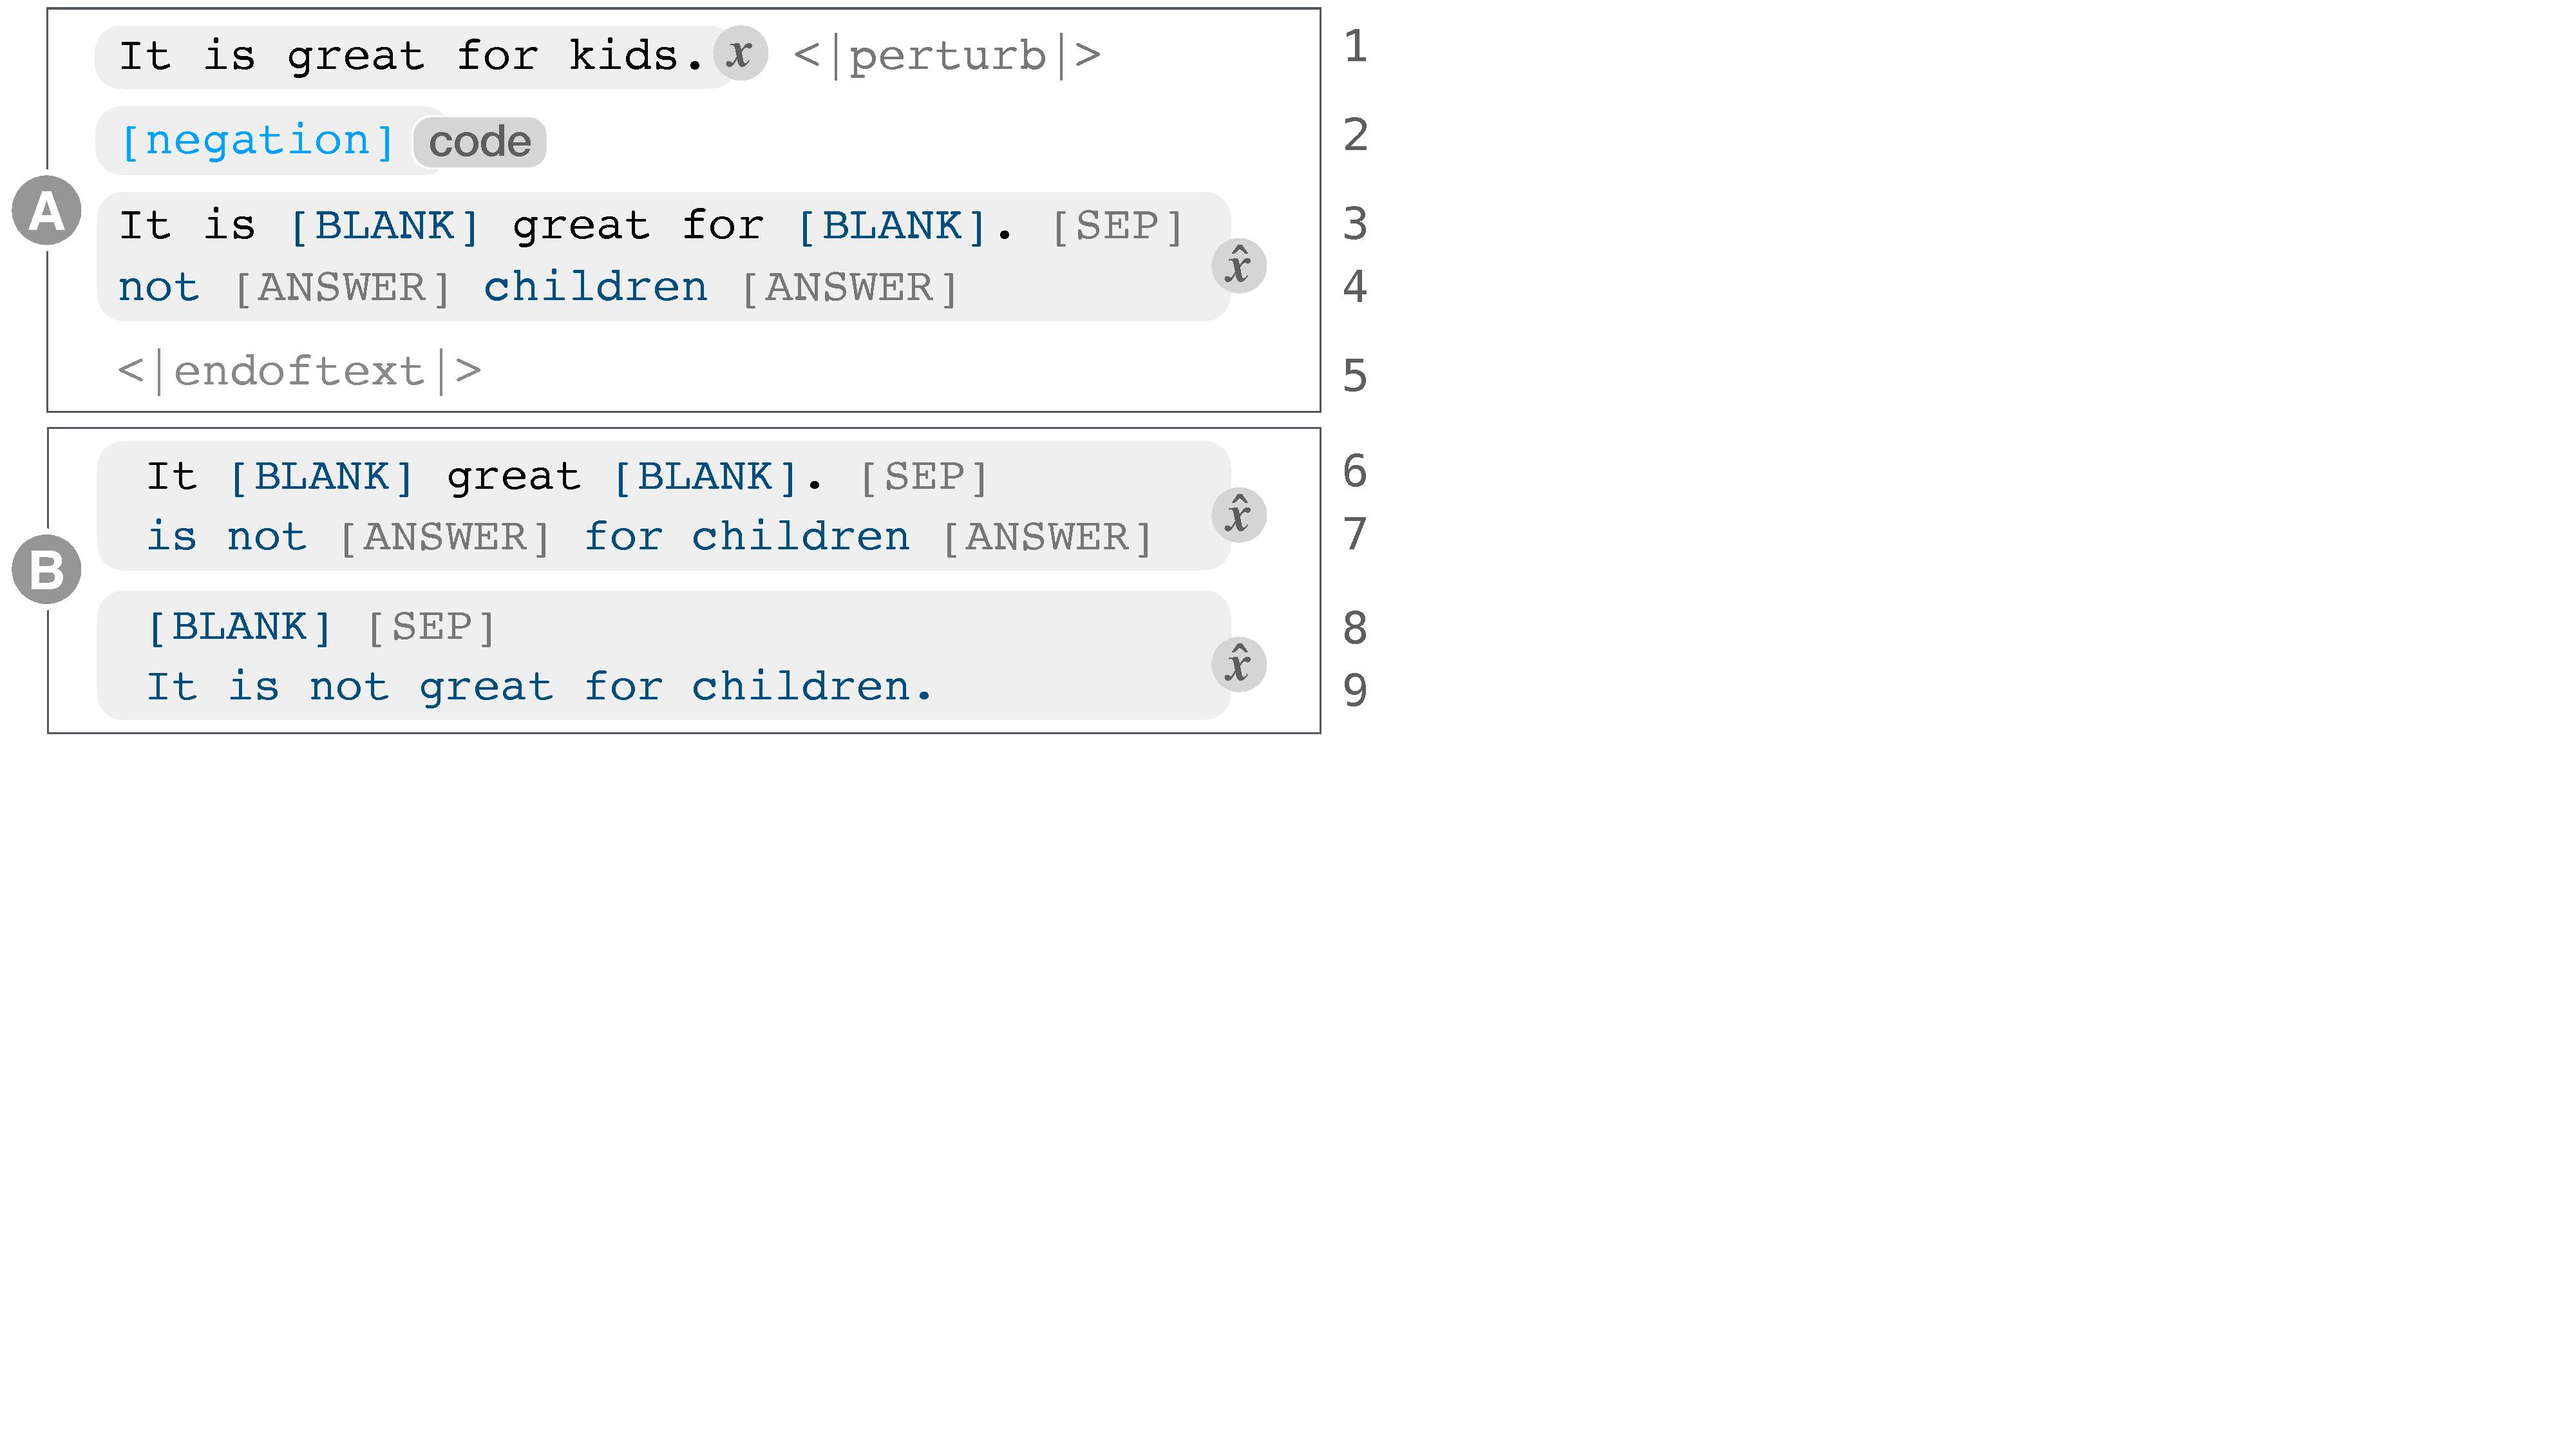
\includegraphics[trim={0 30.7cm 53.2cm 0cm}, clip, width=1\columnwidth]{figures/blank.pdf}
\vspace{-15pt}
\caption{Given a pair of sentences $(x, \xp)$, we generate multiple training prompts with (A) a primary \tagstr, and various blanking strategies, from (B) just the changed tokens, (C) the subtrees, (D) the merged changes, and (E) the entire sentence.\wts{label x and x'; separate the figures.}
%We concatenate the information with special tokens like \perturbtoken.
}
\vspace{-10pt}
\label{fig:blank}
\end{figure}

\subsection{Modeling through Text Generation}
\label{subsec:nlg}

We frame counterfactual generation as a text generation task using language models (LMs).
As we demonstrate in an intrinsic evaluation (\S\ref{appendix:intrinsic}), large pre-trained LMs like GPT-2~\cite{radford2019language} are capable of generating \emph{fluent} text, and are more flexible than word substitutions~\cite{garg2019counterfactual} and templates~\cite{ribeiro2018sear, wu2019errudite} (\ie allow for better \emph{diversity}). 
We detail how we finetune GPT-2 to generate $\xp$ that are \emph{close} to an original instance $x$ (rather than arbitrary text), with control over the $\relation{\xp}$ relationship.
% Here, instead of their common use case, \ie generating the remaining paragraphs, 
% Pre-trained on a large number of web pages curated and filtered by humans, LMs like GPT-2~\cite{radford2019language} naturally generate more \emph{fluent} and \emph{diverse} counterfactuals compared to templates~\cite{ribeiro2018sear} or perturbation functions~\cite{wu2019errudite}.
% We use the original sentence $x$ as the prompt, and finetune off-the-shelf LMs to generate $\xp$: \exinline{$x$ \perturbtoken $\xp$ \stoptoken}.

\paragraph{Controlling counterfactual generation.}
To achieve control over $\relation{\xp}$, we need to be able to control where in $x$ the perturbation happens. 
We extend the Infilling by Language Modeling (ILM) framework~\cite{donahue2020enabling}, such that $x$ is always part of the prompt, and $\xp$ contains \texttt{[BLANK]} tokens where perturbations are to be applied (see Figure~\ref{fig:blank}). 
ILM allows for perturbations of any length (additions and deletions) beyond single word substitutions, \eg Figure~\ref{fig:blank}C--E.

We add another layer of control over relationships by conditioning the generation on special \tagstrs~\cite{raffel2019exploring, Dathathri2020Plug}, \eg \ctrltag{negation} in Figure \ref{fig:blank}A.
Inspired by prior work categorizing manually created counterfactuals~\cite{kaushik2019learning, gardner2020contrast}, we design 8 \tagstrshorts (Table~\ref{table:ctrltag}) that distinguish lexical, syntactic and semantic perturbations. 
We verify through an ablation study in \S\ref{appendix:ablation_control} that training \sysname with \tagstrs greatly improves the success rate when generating counterfactuals that have these properties (by $29\% \pm 18\%$). 

As Figure \ref{fig:blank} indicates, we can control the counterfactual generation conditioning exclusively on $x$ (in which case \sysname selects the \tagstr and the location of \texttt{[BLANK]} tokens) , conditioning on $x$ and the \tagstr, or specifying both the \tagstrshort and where the perturbations happen.

% To specify the perturbation strategy, we condition the generation on special \tagstrs (similar to \citet{raffel2019exploring, Dathathri2020Plug}).
% The 8 \tagstrs in Table~\ref{table:ctrltag} are summarized from 33 papers on textual counterfactual applications.
% We design them to distinguish the information change, with \eg \ctrltag{negation} constraining on concrete behaviors, and \ctrltag{lexical} loosely denoting changes on unigrams or prepositions.
% We further maximize the syntactic differences (\eg \ctrltag{resemantic}, \ctrltag{insert}, or \ctrltag{restructure}), such that the controls are more explicit to follow for the model than semantic-oriented ones (synonyms, antonyms, paraphrases).
% For a given pair $s(x, \xp)$, we compute the primary \tagstrshort based on linguistic features like part-of-speech tags or dependency trees.
% As in Figure~\ref{fig:blank}, we put \tagstrs before the blanked $\xp$ to prioritize \emph{how} over \emph{where}, such that when given a \tagstr, the model can determine the appropriate changing places, and generate the blanked prompt on its own. 



% We further modify the training prompts to allow targeted perturbations, as in Figure~\ref{fig:blank}.
% Besides boosting diversity on top of LMs, the targeted perturbations enable new forms of downstream applications like interactive explanation~\cite{miller} and slice-based data augmentation~\cite{chen2019slice}.

% \emph{Where-to-perturb, with \texttt{[BLANK]}}.
% To perturb specific parts of $x$, We borrow the blank fill-in structure~\cite{donahue2020enabling}, \ie targeted subphrases are replaced with special \texttt{[BLANK]} tokens, and the actual content (``answers'' to blanks) are concatenated to the end. 
% To allow flexible blanking at the generation time, we extend the blank in training prompts to cover the associated parsing structures of edited spans.
%As a result, we form up to four unique training prompts given one $(x, \xp)$ pair.

% \emph{How-to-perturb, with \tagstrs}.
% To specify the perturbation strategy, we condition the generation on special \tagstrs (similar to \citet{raffel2019exploring, Dathathri2020Plug}).
% The 8 \tagstrs in Table~\ref{table:ctrltag} are summarized from 33 papers on textual counterfactual applications.
% We design them to distinguish the information change, with \eg \ctrltag{negation} constraining on concrete behaviors, and \ctrltag{lexical} loosely denoting changes on unigrams or prepositions.
% We further maximize the syntactic differences (\eg \ctrltag{resemantic}, \ctrltag{insert}, or \ctrltag{restructure}), such that the controls are more explicit to follow for the model than semantic-oriented ones (synonyms, antonyms, paraphrases).
% For a given pair $s(x, \xp)$, we compute the primary \tagstrshort based on linguistic features like part-of-speech tags or dependency trees.
% As in Figure~\ref{fig:blank}, we put \tagstrs before the blanked $\xp$ to prioritize \emph{how} over \emph{where}, such that when given a \tagstr, the model can determine the appropriate changing places, and generate the blanked prompt on its own. 
%However, in cases where it is more essential to inspect particular subphrases, it is possible to reverse the order.
%, so we can provide the blanked prompts, and let the model figure out the \emph{how}.
%It is also possible to swap the order of the blanked $\xp$ and the \tagstrs. 

%, we found WordNet~\cite{miller1998wordnet} or sentence similarity based tagging are inaccurate, and the pattern was tricky to learn for the LM model.
%The \tagstrs distinguish the information change: the syntax-preserving ones add (\ctrltag{insert}), remove (\ctrltag{delete}), or change constraints, and the constraints vary from sparse (\ctrltag{resemantic} is more loose than \ctrltag{lexical}) to specific and finer-grained (\ctrltag{negation}, \ctrltag{quantifier}).
%Remaining \ctrltag{shuffle} and \ctrltag{restructure}, on the other hand, focuses on syntactic understanding when we have high lexical overlap.

%\wts{Add some more explanation on the design rationale. It is a more syntactic style change, and we try to minimize the overlaps between words; But we leave out the semantic ones because they overlap too much. arguably lexical and resemantic are similar, but we separate them because editing distance and because too many prior work do lexical change that it deserves a separate category.}

\paragraph{Finetuning dataset.}
We rely on six datasets of paired sentences, each of which contains counterfactuals with a subset of $\relation{\xp}$ relationships of interest (see Table~\ref{table:ctrltag}). 
To increase diversity, we also use heuristics on editing distance to find naturally occurring pairs in non-paired datasets like SQAuD~\cite{rajpurkar-etal-2016-squad}.
A combination of these datasets yields a finetuned model that can produce \emph{diverse} counterfactuals.
For each paired $(x, \xp)$, we create various training prompts as in Figure~\ref{fig:blank}.
We vary the location of \texttt{[BLANK]}s according to the example's parse tree, and compute the primary \tagstrshort based on linguistic features such as part-of-speech tags or dependency trees.
We use the pairs as negative samples if the change is too extensive.
We form $657,144$ training prompts from $191,415$ sentence pairs. 
More dataset details and \tagstrshort statistics are in \S\ref{appendix:train_data}.

% For a given pair $s(x, \xp)$, we compute the primary \tagstrshort based on linguistic features like part-of-speech tags or dependency trees.

% While we do not have a single training set for counterfactual generation, multiple existing datasets contain pair sentences that can be seen as \emph{close} counterfactuals of each other. 
% We combined six such datasets.
% They all contain natural sentences (\eg WinoGrande~\cite{sakaguchi2019winogrande} for Commonsense tasks, PAWS~\cite{zhang2019paws} for paraphrasing) such that the finetuned model still maintain \emph{fluent} generation.
% Moreover, they each expresses a subset of the strategies, and therefore achieves fair coverage on all \tagstrs when combined.
% In total, we collected 657,144 training prompts from 191,415 sentence pairs.
% We list the representative datasets in Table~\ref{table:ctrltag}, and describe the datasets and the finetuning details in \S\ref{appendix:train_data}.


\paragraph{Filtering for fluency.}
Certain combinations of \tagstrs and \texttt{[BLANK]} tokens cause \sysname to generate ungrammatical or nonsensical counterfactuals. 
Similar to the language model constraints used by \citet{morris2020textattack}, we score both $x$ and $\xp$ using GPT-2, and filter out $\xp$ if its log-probability (either on the full sentence or on the perturbed chunks) decreases more than 10 points relative to $x$.
We verify the impact of the filtering through human evaluation, as part of the labeling task in \S\ref{sec:app_label}.
As show in \S\ref{subsec:label_efficiency}, it removes a large portion of unrealistic counterfactuals.

%(though their other constraints may also be useful.)


\paragraph{Using counterfactuals.}
\sysname is general-purpose and task-agnostic, and generates a variety of counterfactuals given one $x$. The most natural way to use \sysname is to generate $\hat{\xset}$ without constraints, and then rank the counterfactuals in  $\hat{\xset}$ according to what is most appropriate for the task at hand (we provide examples of ranking functions for labeling and explanations in  \S\ref{sec:app_label} and \S\ref{sec:app_explain}). However, users can also make use of the various control mechanisms, \eg generating counterfactuals by perturbing only specific subtrees of interest (an example is given in \S\ref{subsec:gen_counterfactual_for_labeling}).


% As a general-purpose and task-agnostic model, our generator does not distinguish counterfactual applications.
% Rather, it (targetedly) generates a large amount of counterfactuals with different combinations of \tagstrs and blanks, and the generated $\hat{\xset}$ should be further selected or ranked based on the relationship $\relation{\xp}$.
% For example, we find adversarial examples with common filtering constraints (\eg sentence semantic similarity~\cite{morris2020textattack}).
% We demonstrate different selections in \S\ref{sec:app_label} and \S\ref{sec:app_explain}.


%pr["pr_sent"]<=10 and pr["pr_phrase"] <=10
%Perplexity is instantiating; Language modeling as an approximation because it measures real world distribution.


